%% =====================================================================
%%  Supplementary Material
%%  Significance filtering induces denominator selection bias in
%%  local genetic correlation
%%  Submission to Genetic Epidemiology (Wiley) -- Supporting Information
%%
%%  Build:  pdflatex supplementary  (x2)
%% =====================================================================
\documentclass[11pt,a4paper]{article}

\usepackage[margin=2.5cm]{geometry}
\usepackage{amsmath,amssymb,bm}
\usepackage{booktabs}
\usepackage{array}
\usepackage{graphicx}
\usepackage[colorlinks=true,allcolors=blue]{hyperref}

\newif\iffigures
\figurestrue
\graphicspath{{figures/}}

\newcommand{\rh}{\hat{\rho}}
\newcommand{\Om}{\bm{\Omega}}
\newcommand{\Sig}{\bm{\Sigma}}
\newcommand{\Slocus}{S_{\mathrm{loc}}}
\newcommand{\Ilocus}{I_{\mathrm{loc}}}
\newcommand{\re}{r_{\mathrm{e}}}
\newcommand{\crf}{c_{\mathrm{ref}}}
\newcommand{\Nref}{N_{\mathrm{ref}}}

\renewcommand{\thetable}{S\arabic{table}}
\renewcommand{\thefigure}{S\arabic{figure}}
\renewcommand{\theequation}{S\arabic{equation}}
\renewcommand{\thesection}{S\arabic{section}}

\title{Supplementary Material\\[4pt]
\large Significance filtering induces denominator selection bias in local genetic
correlation: closed-form characterization, a gate-aware correction, and an applicability
diagnostic}
\author{Dana Paquin$^1$, Riddhiman Jain$^2$ \\[0.5em]
{\small $^1$Stanford University; $^2$Independent Researcher, Ahmedabad, India}}
\date{}

\begin{document}
\maketitle

\noindent This Supporting Information file contains Supplementary Methods S1--S3, Supplementary Tables
S1--S3 and Supplementary Figure S1, referenced from the main text. Every number is
generated by the deposited code; none is entered by hand.

\medskip
\noindent\textbf{Use of AI tools.} The authors used large language models to edit the text
of this document and to help write the verification code referenced throughout (for
example \path{code/replication/V0_exactness_check.R} and \path{code/R/test_lavagate.R}).
No section of the text, and no table or figure, was taken from a model's output without
the authors' own revision. All code was read and checked by the authors, and every number
reported here is regenerated by the deposited scripts rather than entered by hand. The
authors are responsible for the whole of the content.

\tableofcontents

%% =====================================================================
\section{The exact moment identities, and their implementation}
%% =====================================================================

The derivation of Section~2.3 of the main text needs two quantities for a noncentral
$\chi^2$ variate: the probability that it exceeds the gate threshold, and its first moment
truncated to that region. Both are available in closed form, so the correction contains no
numerical integration.

\paragraph{The Poisson mixture.} A noncentral chi-square with $m$ degrees of freedom and
noncentrality $\lambda$ is a Poisson-weighted mixture of central chi-squares,
\begin{equation}
\chi'^2_m(\lambda) \;=\; \sum_{j\ge0} \mathrm{Pois}(j;\lambda/2)\,\chi^2_{m+2j},
\end{equation}
so any functional of the noncentral law that is available for the central law is available
for the noncentral one by summing a rapidly convergent series. In our implementation the
series is truncated where the weight falls below $10^{-14}$ of its maximum, with the index
bounded by $\lambda/2 + 12\sqrt{\lambda/2}$.

\paragraph{The truncated first moment.} For a central chi-square,
\begin{equation}
E\bigl[\chi^2_m\,\mathbf{1}\{\chi^2_m > t\}\bigr] \;=\; m\,P(\chi^2_{m+2} > t),
\end{equation}
which follows in one line by absorbing the extra factor of $x$ into the density. Since
$f_m(x)\propto x^{m/2-1}e^{-x/2}$, we have $x\,f_m(x) = m\,f_{m+2}(x)$.

Combining the two gives the gate pass probability and the truncated first moment of
$S_{ii}$ exactly. Writing $t=\chi^2_{K,\,0.95}$ and $\lambda_i = K\theta_i$,
\begin{equation}
\Delta_i \;=\; E[S_{ii}\mid S_{ii}>t] - E[S_{ii}]
\end{equation}
is the gate-induced inflation of the $i$th diagonal used throughout the main text.
It conditions on trait $i$'s own gate. The reported gate conditions on both, and the
two diagonals are dependent whenever $\re\neq0$, with
$\mathrm{Cov}(S_{11},S_{22})=2K(\re^2+2\re\Omega_{12})$, so $\Delta_i$ is exact at
$\re=0$ and accurate to second order in $\re$ otherwise.

\paragraph{The reference-size correction.} $\crf = (\Nref-K-1)/(\Nref-1)$ is written, named
and applied at three separate points of the LAVA source, but \texttt{nref.correction} is
assigned \texttt{FALSE} inside the body of \texttt{process.locus()}
(\texttt{input\_processing.R:38}), is not exposed as a parameter, and cannot be set by the
caller. In v0.1.5 it therefore evaluates to exactly 1 and the correction is inert. We
retain the general form in the main text because it is what the code expresses and what a
reimplementation would apply. At $K=270$ and $\Nref=99{,}339$ the intended factor is
0.99727, so the distinction shifts the gate threshold by 0.27\% and no quantity reported
in the paper depends on it. Tier~B, running through LAVA's own code path, already reflects
$\crf = 1$.

\paragraph{Cross-implementation check.} The R module \texttt{code/R/lavagate.R} and the
Python used for every number in the paper are independent ports of the same closed form.
They are checked against each other on 500 parameter combinations spanning
$K\in[50,500]$, $\theta\in[0.005,0.30]$ and $\re\in[0,0.20]$, agreeing to
$1.3\times10^{-12}$ on $\Delta$ and $1.8\times10^{-15}$ on the slope and intercept
(\texttt{code/R/test\_lavagate.R}).

%% =====================================================================
\section{Verification of the attribution control}
%% =====================================================================

The Tier~C control of Section~2.5 evaluates the gate statistic and $\rh$ directly rather
than through \texttt{run.univ()} and \texttt{run.bivar()}, which would be infeasible at
the replicate count required. That substitution is legitimate only if the direct formulas
are LAVA's, so we verify it rather than assert it, by pushing identical $\bm{\delta}$
matrices through both paths and comparing them.

Over 5,000 replicates spanning $K\in[39,584]$ and $\re\in[0,0.24]$, agreement is exact, at
a maximum relative difference of 0 on all 10,000 univariate $P$-values and all 1,909
defined $\rh$ values, after applying the \texttt{signif(., 6)} rounding LAVA applies to its
own output. The same run confirms the nesting of main-text Section~2.1 empirically. Of 148
gate passes, zero had a non-positive denominator, and all 2,322 \texttt{run.bivar()} aborts
were loci that were not estimable.

Because the simulation depends on a locus only through $(K,\theta_1,\theta_2,\re)$, since
both $\rh$ and $U_i$ are invariant to rescaling $\Sig$ and $\Om$ together, the control
uses the real per-locus values measured by Tier~B, at twice its replicate count. The
verification is deposited as \path{code/replication/V0_exactness_check.R}, which is a
precondition for \path{V1_gate_attribution.R} and exits non-zero if agreement is not
exact.

%% =====================================================================
\section{One genome pass per pair, and why not one pass for the panel}
%% =====================================================================

\texttt{process.locus()} returns $\Om$ and $\Sig$ for every phenotype in its input object,
so a single genome pass over all eight phenotypes would in principle serve all six pairs at
a sixth of the compute. Three mechanisms make $K$ depend on the phenotype set, and the
third is decisive.

Two do not bind at this panel's sample sizes. The cap
$\texttt{max.K} = \lfloor \texttt{max.prop.K}\cdot\min(N)\rfloor$ evaluates to 34,762 for
the smallest study (ASD, $N=46{,}350$) against a largest observed $K$ of 607, and the rule
that nulls $h^2$ when $K/N > 0.1$ is far from triggered at $K/N = 0.013$.

The third binds. \texttt{process.input()} reduces every phenotype to the SNPs common to
\emph{all} phenotypes in the object and the reference panel. Measured on the harmonized
panel, ASD $\times$ SCZ with the reference retains 5,774,835 SNPs, whereas all eight
phenotypes retain 2,306,339. Since $K$ is close to proportional to the number of SNPs in a
block, and the univariate noncentrality is $K\theta$, a combined pass would not merely be
less precise. It would alter the attrition cascade it exists to measure, and the
completed pair would not reproduce its own published numbers.

Each pair is therefore run in its own pass, at its own two-trait SNP intersection, with one
exception. P2a and P2b are run together, in a single four-phenotype pass, because the two
PGC releases have genuinely different SNP coverage and running the arms separately would
add a second difference between them and destroy the control. Sharing one pass forces the
identical SNP set on both arms, at the cost of a smaller SNP set for P2 alone. Because
\texttt{process.locus()} drops phenotypes individually, a locus in that pass can be
analysable for one arm and not the other, so the surviving phenotype set is recorded per
locus and each arm is scored independently against it.

%% =====================================================================
\section{Supplementary tables}
%% =====================================================================

\begin{table}[htbp]
\centering
\caption{\textbf{Where loci and phenotypes are lost.} Five mechanisms, identified by
tracing each loss on real data back to the LAVA v0.1.5 source. Channels 2 and 5 are wholly
undocumented; channel 4 is documented in part.}
\label{tab:S1}
\small
\begin{tabular}{@{}p{0.4cm}p{2.6cm}p{7.9cm}p{1.6cm}@{}}
\toprule
\# & Mechanism & Location and effect & Documented \\
\midrule
1 & Locus not processed & \texttt{process.locus()} returns \texttt{NULL}: insufficient SNPs
after harmonisation, or \emph{all} phenotypes have negative local variance & Yes \\[2pt]
2 & Phenotype discarded & \path{input_processing.R:169--171}: negative local variance
for one trait, or an \texttt{NA} from $N<K$ or inversion failure; that trait is silently
removed and the locus returned as if analysable & \textbf{No} \\[2pt]
3 & The univariate filter & \texttt{analysis\_functions.R:42--44}: both traits must clear
$P<0.05$ & Yes \\[2pt]
4 & Parameter truncation & \texttt{analysis\_functions.R:384--385}: $\rh$ set to
\texttt{NA} when $|\rh| > \texttt{param.lim}$ (default 1.25); survivors then capped to
$[-1,1]$ at line 174 & Partly \\[2pt]
5 & \texttt{run.bivar()} aborts & \texttt{analysis\_functions.R:375}, then 387: on a locus
with a negative local variance, \texttt{estimate.params()} returns \texttt{NaN} and
\texttt{filter.params()} evaluates \texttt{if (any(NA))}, raising \emph{``missing value
where TRUE/FALSE needed''} & \textbf{No} \\
\bottomrule
\end{tabular}
\end{table}

\noindent Channel 2 is the consequential one and is quantified per pair in main-text
Table~6. Channel 5 is reported for what it implies rather than for how often it bites.
\texttt{run.bivar()} does not return \texttt{NA} for a locus it cannot analyse, it raises
an error and halts. Users never meet this, because \texttt{run.univ.bivar()} only reaches
the bivariate step through the filter, and the filter guarantees a positive denominator.
The filter is therefore load-bearing for the pipeline to run at all, not an optional
stabiliser that could simply be switched off. Channel 4 is a filter on the answer rather
than on the data, and its two stages are often conflated. \texttt{param.lim} discards
$|\rh| > 1.25$ entirely, while \texttt{cap.estimates} silently rewrites $|\rh|$ between 1
and 1.25 to exactly $\pm1$.

\vspace{1em}

\begin{table}[htbp]
\centering
\caption{\textbf{Closed form against Tier~A Monte Carlo}, 200,000 loci per cell. Mean
relative error on the slope is 1.14\% and the maximum 2.06\%; maximum absolute error on
the intercept is 0.0052. The closed form returns an intercept of exactly zero when
$\re = 0$, as it must.}
\label{tab:S2}
\small
\begin{tabular}{@{}lrrrrrrr@{}}
\toprule
& & & \multicolumn{3}{c}{Attenuation slope} & \multicolumn{2}{c}{Intercept} \\
\cmidrule(lr){4-6}\cmidrule(lr){7-8}
Scenario & $K$ & $\re$ & simulated & closed form & rel.\ diff.\ & simulated & closed form \\
\midrule
S1 asymmetric power & 300 & 0.00 & 0.6064 & 0.6133 & 1.15\% & 0.0047 & 0.0000 \\
S2 matched moderate & 300 & 0.00 & 0.5721 & 0.5787 & 1.16\% & 0.0041 & 0.0000 \\
S3 overlap $\re=0.05$ & 300 & 0.05 & 0.6062 & 0.6133 & 1.18\% & 0.0378 & 0.0339 \\
S4 overlap $\re=0.10$ & 300 & 0.10 & 0.6010 & 0.6133 & 2.06\% & 0.0709 & 0.0677 \\
S5 small $K$ & 100 & 0.00 & 0.4507 & 0.4555 & 1.06\% & 0.0016 & 0.0000 \\
S6 large $K$ & 500 & 0.00 & 0.6880 & 0.6897 & 0.25\% & 0.0052 & 0.0000 \\
\bottomrule
\end{tabular}
\end{table}

\noindent Against 42 held-out configurations not used in its construction, the
second-order form of main-text Section~2.3 achieves a mean absolute error of 0.0066 and a
maximum of 0.0348, with 88\% of cells within 0.01. The leading-order, denominator-only form
achieves 0.0492 and 0.1709 on the same cells. The slope varies with $K$ even at fixed
heritability, from 0.4555 at $K=100$ to 0.6897 at $K=500$, which is the first indication
that a single genome-wide correction factor cannot be right.

\vspace{1em}

\begin{table}[htbp]
\centering
\caption{\textbf{Interval coverage, width and sign determinacy.} Top: coverage and width
before and after the filter, against the real data. Bottom: the fraction of simulated
intervals excluding zero as a function of true $\rho$, showing near-symmetry in the sign of
$\rho$.}
\label{tab:S3}
\small
\begin{tabular}{@{}lrrr@{}}
\toprule
& Coverage & Mean width & Fraction wider than 1 \\
\midrule
Simulated, pre-filter  & 0.974 & 1.651 & 0.936 \\
Simulated, post-filter & 0.949 & 1.386 & 0.869 \\
Real data, P4          & ---   & 1.365 & 0.859 \\
\bottomrule
\end{tabular}

\vspace{0.8em}

\begin{tabular}{@{}rrr@{}}
\toprule
True $\rho$ & Spans zero & Sign determinate \\
\midrule
$-0.4$ & 0.861 & 0.139 \\
$-0.2$ & 0.915 & 0.085 \\
$0.0$  & 0.937 & 0.063 \\
$+0.2$ & 0.920 & 0.080 \\
$+0.4$ & 0.877 & 0.123 \\
$+0.6$ & 0.779 & 0.221 \\
\bottomrule
\end{tabular}
\end{table}

\noindent Post-filter coverage is 0.949 against a nominal 0.950, so the filter does not
break calibration. Determinacy at $\rho=-0.4$ (0.139) and $\rho=+0.4$ (0.123) is
near-identical, so the \emph{count} of sign-determinate loci cannot discriminate between a
diametric and a convergent architecture, while their \emph{direction} can. Sample overlap
breaks the symmetry, raising determinacy on the positive arm only, which is why the sign
test of the main text uses the filtered null rather than a 50/50 binomial.

\clearpage
%% =====================================================================
\section{Supplementary figure}
%% =====================================================================

\begin{figure}[htbp]
\centering
\iffigures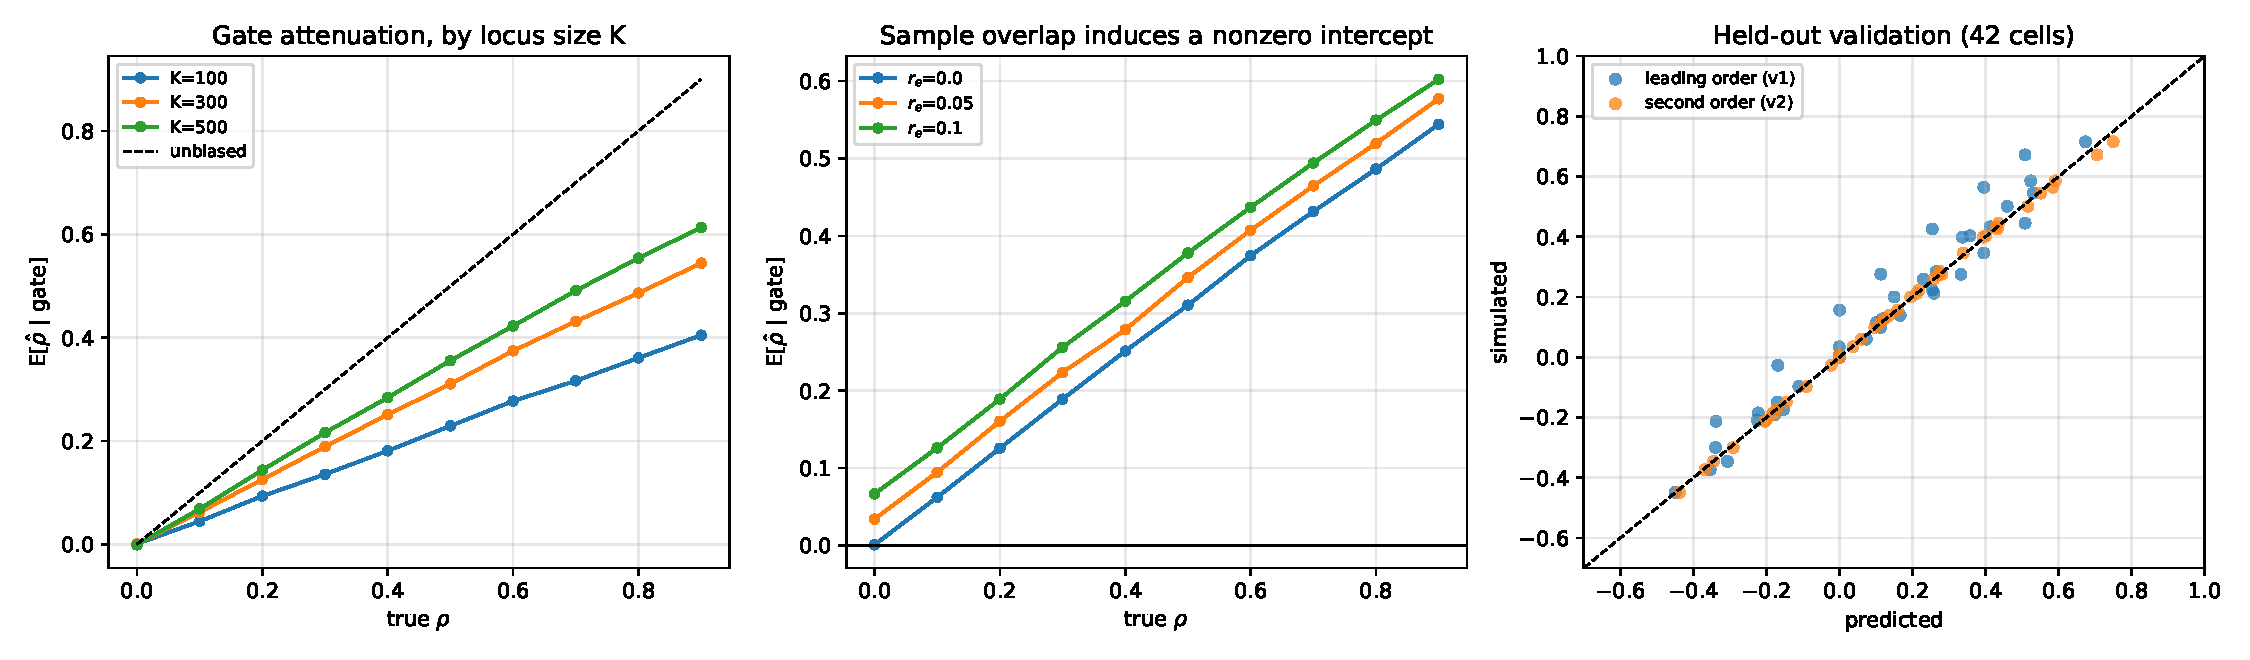
\includegraphics[width=\linewidth]{FigureS1_tierA_diagnostics}\fi
\caption{\textbf{Tier~A diagnostics for the closed-form derivation.} Attenuation of
$E[\rh\mid G]$ against true $\rho$ at three locus sizes $K$, the same at three levels of
sample overlap, and held-out validation of the second-order form against the
leading-order one on 42 parameter cells. All panels are sampling-model simulation at
200,000 loci per cell.}
\label{fig:S1}
\end{figure}

\end{document}
